\documentclass[../main.tex]{subfiles}
\begin{document}
\chapter{Soluzione proposta}
\paragraph{Preparazione environment}
Per lo sviluppo del programma e lo studio del framework è stata creata una piattaforma dedicata alla \textit{Security Analytics}. L'installazione verrà effettuata su \textit{virtual machine} dedicata con Ubuntu 16.04 LTS.

\section{Installazione Stratosphere IPS}
Sulla macchina virtuale è stato installato il framework di Stratospehere IPS. Per l'installazione si sono seguiti i seguenti passaggi:

\begin{itemize}
				\item Installazione del programma git \textit{2.7.4}
\begin{lstlisting}[language=bash]
$ sudo apt install git
\end{lstlisting}

				\item Clonazione repository github del framework
\begin{lstlisting}[language=bash]
$ git clone https://github.com/stratosphereips/StratosphereTestingFramework
\end{lstlisting}

				\item Installazione del programma \textit{python-pip}
\begin{lstlisting}[language=bash]
$ sudo apt install python-pip
\end{lstlisting}
\end{itemize}
				
\begin{itemize}
				\paragraph{Installazione dipendenze per Stratosphere IPS}

				\item prettytable \textit{0.7.2-3}
\begin{lstlisting}[language=bash]
$ sudo apt install python-prettytable
\end{lstlisting}

				\item transaction \textit{1.4.3-3}
\begin{lstlisting}[language=bash]
$ sudo apt install python-transaction
\end{lstlisting}

				\item persistent \textit{4.1.1-1build2}
\begin{lstlisting}[language=bash]
$ sudo apt install python-persistent
\end{lstlisting}

				\item zodb \textit{5.4.0}
\begin{lstlisting}[language=bash]
$ sudo pip install zodb
\end{lstlisting}

				\item sparse \textit{1.1-1.3build1}
\begin{lstlisting}[language=bash]
$ sudo apt install python-sparse
\end{lstlisting}

				\item dateutil \textit{2.4.2-1}
\begin{lstlisting}[language=bash]
$ sudo apt install python-dateutil
\end{lstlisting}


\end{itemize}

\section{Installazione di Argus}

\begin{itemize}
				\item libpcap \textit{1.7.4-2}
\begin{lstlisting}[language=bash]
$ sudo apt install libpcab-dev
\end{lstlisting}

\item bison \textit{3.0.4}
\begin{lstlisting}[language=bash]
$ sudo apt install bison
\end{lstlisting}

\item flex \textit{2.6.0-11}
\begin{lstlisting}[language=bash]
$ sudo apt install flex
\end{lstlisting}

\item Installazione dell'ultima versione di argus \textit{3.0.8.2} dal sito http://qosient.com/argus/dev/argus-latest.tar.gz

\item Installazione dell'ultima versione di argus-client \textit{3.0.8.2} dal sito http://qosient.com/argus/dev/argus-clients-latest.tar.gz

\end{itemize}

\section{Utilizzo del programma stf\\}
Per eseguire il programma lo si esegue con
\begin{lstlisting}[language=bash]
	./stf.py
\end{lstlisting}

Per caricare un dataset si utilizza il comando
\begin{lstlisting}[language=bash]
	datasets -c /absolute/path/file.binetflow	
\end{lstlisting}

Per generare la connessione si utilizza il comando
\begin{lstlisting}[language=bash]
	connections -g	
\end{lstlisting}

Infine, per generare i modelli, il comando
\begin{lstlisting}[language=bash]
	models -g	
\end{lstlisting}

Per visualizzare il behavioral model si utilizza il comando
\begin{lstlisting}[language=bash]
	models -L [id]	
\end{lstlisting}
\end{document}


La scrittura del programma è stata effettuata in due fasi, nella prima è stato realizzato un programma che effettua la conversione in single core. Nella seconda fase si è passati alla parallelizzazione del programma.

\section{Conversione}
I due formati che vengono utilizzati hanno formati diversi, si è scelto di tenere soltanto i campi utilizzati dal programma \textit{Argus} poichè è il formato che viene utilizzato da Stratosphere. I campi di \textit{nProbe} che quindi non compaiono nei file di tipo \textit{*.binetflow} vengono scartati.

Per i restanti campi si rimanda alla seguente tabella di conversione
\begin{table}[H]
				\centering
				\caption{Tabella di conversione}
				\label{Tabella di conversione}
				\begin{tabular}{|l|l|}
								\hline
								binetflow												 & flow																								 \\ \hline
								start time											 & first switched																			 \\ \hline
								duration												 & last switched - first switched											 \\ \hline
								protocol												 & protocol																						 \\ \hline
								source address                   & ipv4 source address                                 \\ \hline
								source port                      & source port                                         \\ \hline
								direction                        & biflow direction                                    \\ \hline
								destination address              & ipv4 destination address                            \\ \hline
								destination port                 & destination port                                    \\ \hline
								state                            & -                                                   \\ \hline
								source tos                       & source tos                                          \\ \hline
								destination tos                  & -                                                   \\ \hline
								tot packets                      & input packets + output packets                      \\ \hline
								tot bytes                        & input bytes + output bytes                          \\ \hline
								source bytes                     & input bytes                                         \\ \hline
								source data											 & -																									 \\ \hline
								destination data								 & -																									 \\ \hline
								label														 & -																									 \\ \hline

				\end{tabular}
\end{table}

\section{Automatizzazione conversione}
La conversione è stata automatizzata con la scrittura di uno script in \textit{python}. Si è scelto di scrivere un programma usando questo linguaggio per la facilità di utilizzo nel lavorare con i file e per le performance.

Il problema richiede lo sviluppo di un programma che converte file in modalità batch. \newline

Pseudocodice del programma 
\begin{algorithm}
\caption{Single core version}\label{single core version}
\begin{algorithmic}[1]
\Procedure{Hydra}{}
\ForAll{\textit{file} in path}
\State read data from \textit{file}
\State convert data into new format
\State append data into new file
\EndFor

\EndProcedure
\end{algorithmic}
\end{algorithm}

Come descritto nel capitolo 3, i file hanno una struttra gerarchica per data. Si esegue quindi un ciclo \textit{for} che prende tutti i file in modo ricorsivo.

Si è scelto di leggere il file una riga alla volta perchè le grandi dimensioni dei file non permettono un approccio diverso. Un approccio più veloce sarebbe stato quello di leggere i file per intero nella memoria principale ma non è possibile per le grandi dimensioni dei file.
\newline

Per ogni riga che viene letta si elimina il carattere speciale che divide i valori e li si inserisce in un vettore principale. Per ogni riga letta si ha quindi un vettore con posizioni dei campi fissi (es. l'IP sorgente sarà sempre in posizione vettore[0]).
\newline

Si crea un vettore per ogni campo che dovrà essere convertito e dal vettore principale vengono appesi i valori. Successivamente si apre un file nel formato \textit{binetflow} e vengono convertiti e appesi i valori da ogni vettore.

\section{Rendere efficiente la conversione}

Nel programma descritto in precendenza viene generato un solo file di output in cui vengono convertiti tutti i file dati in input. Questa soluzione è comoda perchè da migliaia di file si ha un solo file con i dati convertiti, ma presenta il problema di creare un file con dimensioni enormi e di difficile gestione (il file può raggiungere dimensioni tali da rendere difficile anche solo aprirlo in lettura) su cui crearci i modelli comportamentali.

Il programma è inoltre inefficiente poichè è single core e ha come collo di bottiglia la scrittura su un unico file.

La soluzione proposta seppure sia teoricamente corretta non può avere un'applicazione nel mondo reale. Bisogna cambiare quindi strategia per rendere la conversione più veloce sfruttando le macchine multi core e per avere in output file di dimensioni accettabili.

\subsection{Possibili soluzioni}
Si possono pensare diverse soluzioni che migliorerebbero in modo significativo il programma visto in precedenza. 

\begin{itemize}
				\item Lavorare su chunk di file
				\item Meccanismi di lock
				\item Scrittura su file 1:1
\end{itemize}

\paragraph{Lavorare su chunk di file}
Per velocizzare il programma e sfruttare i processori disponibili si potrebbe assegnare ad ogni processore un file da leggere e convertire. Quando il processore termina la conversione dei dati scrive sul file in output. In questo modo si dividrebbe il tempo di esecuzione sul numero di processori disponibili. 
Questa soluzione rende il più veloce possibile la conversione dei file ma i processori finiscono per scrivere sullo stesso file senza avere nessuna regola di precedenza, questo crea problemi perchè le scritture in output non sono ordinate e non è possibile creare modelli comportamentali affidabili. Le scritture su file devono essere ordinate e sequenziali. Inoltre questa soluzione ha il problema di scrivere sempre su unico file e come detto in precedenza questo tipo di soluzione non è possibile.

\paragraph{Meccanismi di lock}
Un modo per risolvere i problemi precedenti è quello di utilizzare il concetto di semaforo. \newline

In informatica un semaforo è un tipo di dato astratto gestito da un sistema operativo multitasking per sincronizzare l'accesso a risolrse condivise tra processi. È composto da una variabile intera e da una coda di processi. Quando un processo apre il file per scriverci viene impostato un semaforo che segnala che la risorsa è occupata, se un altro processore prova ad aprire lo stesso file per scriverci gli sarà negato l'accesso dal semaforo fino a quando l'altro processo non rilascerà la risorsa.

In questo modo si risolve il problema delle scritture ordinate, ma c'è da tener conto che i semafori riducono la velocità di esecuzione dell'algoritmo poichè mentre un processore occupa la risorsa tutti gli altri processori devono mettersi in coda per aspettarne il rilascio. Questa soluzione sebbene rallenti l'esecuzione del programma rispetto alla soluzione precedente è comunque molto più veloce della versione single core perchè si guadagna comunque molto tempo nella lettura e conversione dei dati che viene effettuata alla massima velocità possibile. Questa soluzione risolve anche il problema dell'ordinamento delle scritture. \newline

Rimane il problema della scrittura su un unico file che però può essere risolto facilmente decidendo di scrivere su un nuovo file quando raggiunge una dimensione specificata.

Se si implementa la divisione del file di output questa soluzione può considerarsi efficiente anche se rimane il collo di bottiglia introdotto dai semafori che costringe i processi ad aspettare in coda quando una risorsa è impegnata.

\paragraph{Scrittura su file 1:1}
In questa soluzione ogni processore apre un file, lo legge. lo converte e scrive la conversione su un proprio file.
Questa soluzione è decisamente la più semplice tra quelle proposte ed è anche la più efficiente poichè i processori non entrano mai in conflitto tra di loro cosicchè da effettuare letture, conversioni e scritture alla massima velocità possibile dalla macchina.
Un problema che può creare questa soluzione è la produzione di una grande quantità di file in output. Si pensi di dover una sola settimana di traffico di rete, sono circa 10 mila file.

\subsection{Scelta effettuata}

Si è scelto di procedere con l'ultima soluzione presentata perchè data la grande quantità di informazioni da convertire si preferisce l'approccio più veloce a discapito dell'ordinamento finale.


Pseudocodice del programma multi core
\begin{algorithm}
\caption{Multi core version}\label{multi core version}
\begin{algorithmic}[1]
\Procedure{Hydra}{}
\ForAll{\textit{file} in path}
\State $\textit{Queue[]} \gets \textit{file}$
\State read data from $\textit{file}$
\State spawn 4 process
\While{\textit{Queue[]} $\textbf{not empty}$}
\State $\textit{filename} \gets $\textit{Queue.get()}
\State convert data into new format
\State append data into new file
\EndWhile
\EndFor
\EndProcedure
\end{algorithmic}
\end{algorithm}
\end{document}

\begin{center}
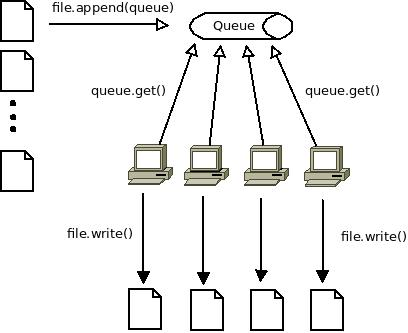
\includegraphics[scale=0.5]{multicore}
\end{center}

Il programma, dato in input la root directory dei file, cerca ricorsivamente tutti i file e li inserisce in una coda, chiama poi una funzione a cui assegna 4 processori. La funzione ha un ciclo while che si ripete fino a quando la coda popolata da tutti i file non è vuota. Ogni processore che entra in questa funzione toglie un file dalla coda e lo elabora. \newline

